\section{Minimum Halo Mass}
\label{sec:halo_mass}

\Contributors{Arka Banerjee, Nilanjan Banik, Keith Bechtol, Ana Bonaca, Kimberly K.\ Boddy, Jo Bovy, Francis-Yan Cyr-Racine, Alex Drlica-Wagner, Ana D{\'i}az Rivero, Cora Dvorkin, Denis Erkal, Christopher D.\ Fassnacht, David Hendel, Yashar D.\ Hezaveh, Charles R.\ Keeton, Sergey Koposov, Ting S.\ Li, Yao-Yuan Mao, Mitch McNanna, Ethan O.\ Nadler, Andrew B.\ Pace, Nora Shipp, Erik Tollerud, Mei-Yu Wang, Risa H.\ Wechsler}

The cold, collisionless model of dark matter makes a strong prediction that dark matter halos should exist down to Earth-mass scales (or below) in WIMP and non-thermal axion models \citep{Green:2003un,2005Natur.433..389D,1412.5930}.
Several modifications to the cold, collisionless dark matter paradigm can suppress the formation of dark matter halos on these small scales.
Current observations provide a robust measurement of the dark matter halo mass spectrum for halos with mass $> 10^{10}\Msun$, and the smallest known galaxies provide an existence proof for halos of mass $\roughly 10^8 \Msun - 10^9 \Msun$ \citep{2017MNRAS.467.2019R,behroozi2018,Jethwa:2018,Kim:2017iwr,Nadler:2018,1807.07093}. 
Extending below this halo mass threshold is challenging due to our limited observational sensitivity to the faintest galaxies.
In addition, halos with mass $\lesssim 10^8 \Msun$ are generally expected to host few (if any) stars \citep{1102.4638,1505.06209}, necessitating novel detection techniques that do not rely on the baryonic content of halos.
Here we explore improvements that LSST will make in measuring the faintest galaxies and in probing dark matter halos below the threshold of galaxy formation with stellar streams and strongly lensed systems. We then use these improvements to forecast constraints on specific dark matter models.

\subsection{Milky Way Satellite Galaxies \Contact{Ethan}} 
\label{sec:smallest_galaxies}
\Contributors{Ethan O.\ Nadler, Keith Bechtol, Alex Drlica-Wagner, Mitch McNanna, Andrew B.\ Pace, Yao-Yuan Mao, Erik Tollerud, Risa Wechsler, Francis-Yan Cyr-Racine, Mei-Yu Wang, Kimberly K.\ Boddy, Arka Banerjee}

% Some slides from KITP Dark Matter Program in May 2018 with potential ideas:
% https://drive.google.com/open?id=1BhuwyNE7vClIeVV6FhM99QtictTvpQ0p

\vspace{1em} \noindent \textbf{The Threshold of Galaxy Formation}

Galaxies are born and grow within dark matter halos.
To first approximation, galaxies with the largest stellar masses reside within the highest-mass dark matter halos, while fainter galaxies---which are much more numerous---occupy dark matter halos with progressively smaller typical masses; however, the scatter between stellar mass and halo mass is likely large in the low-mass regime (see \citealt{Wechsler:2018} for a recent review).
Therefore, the smallest and faintest galaxies offer a natural place to search for extremely low-mass dark matter halos, which are in turn sensitive probes of dark matter microphysics. Another advantage of probing low-mass dark matter halos using faint galaxies is that we can study their properties in detail, \eg, via follow-up spectroscopy (\secref{complementarity}).

The challenge in interpreting observations of faint galaxies is the complex relationship between baryons and halos at this extreme mass scale and the effects of baryonic physics both within subhalos and on subhalo populations as a whole \citep[\eg,][]{DOnghia:2009xhq,Brooks:2012ah,errani2017,Garrison-Kimmel:2017zes,1811.11791,brooks2018}. Nevertheless, probing the extreme faint end of the galaxy luminosity function is valuable both astrophysically and in terms of constraining dark matter models. For example, a driving question for near-field cosmology with LSST is how well we can use the population of Milky Way satellites to constrain the minimum dark matter halo mass necessary for galaxy formation. 
This ``minimum halo mass" depends on the details of reionization and other forms of baryonic feedback that prevent gas from accreting and cooling in low-mass subhalos; however, it might also reflect a cutoff in the subhalo mass function determined by the particle nature of dark matter (\eg, WDM or FDM). In particular, models that produce a cutoff in the matter power spectrum generally suppress the number of subhalos below a characteristic mass threshold (\eqnref{Mhm}). Thus, the existence, abundance, and properties of the smallest galaxies generically lead to constraints on dark matter models that reduce small-scale power.

\vspace{1em} \noindent {\bf Minimum Subhalo Mass Inferred from Milky Way Satellites}

\begin{figure}[t]
\centering
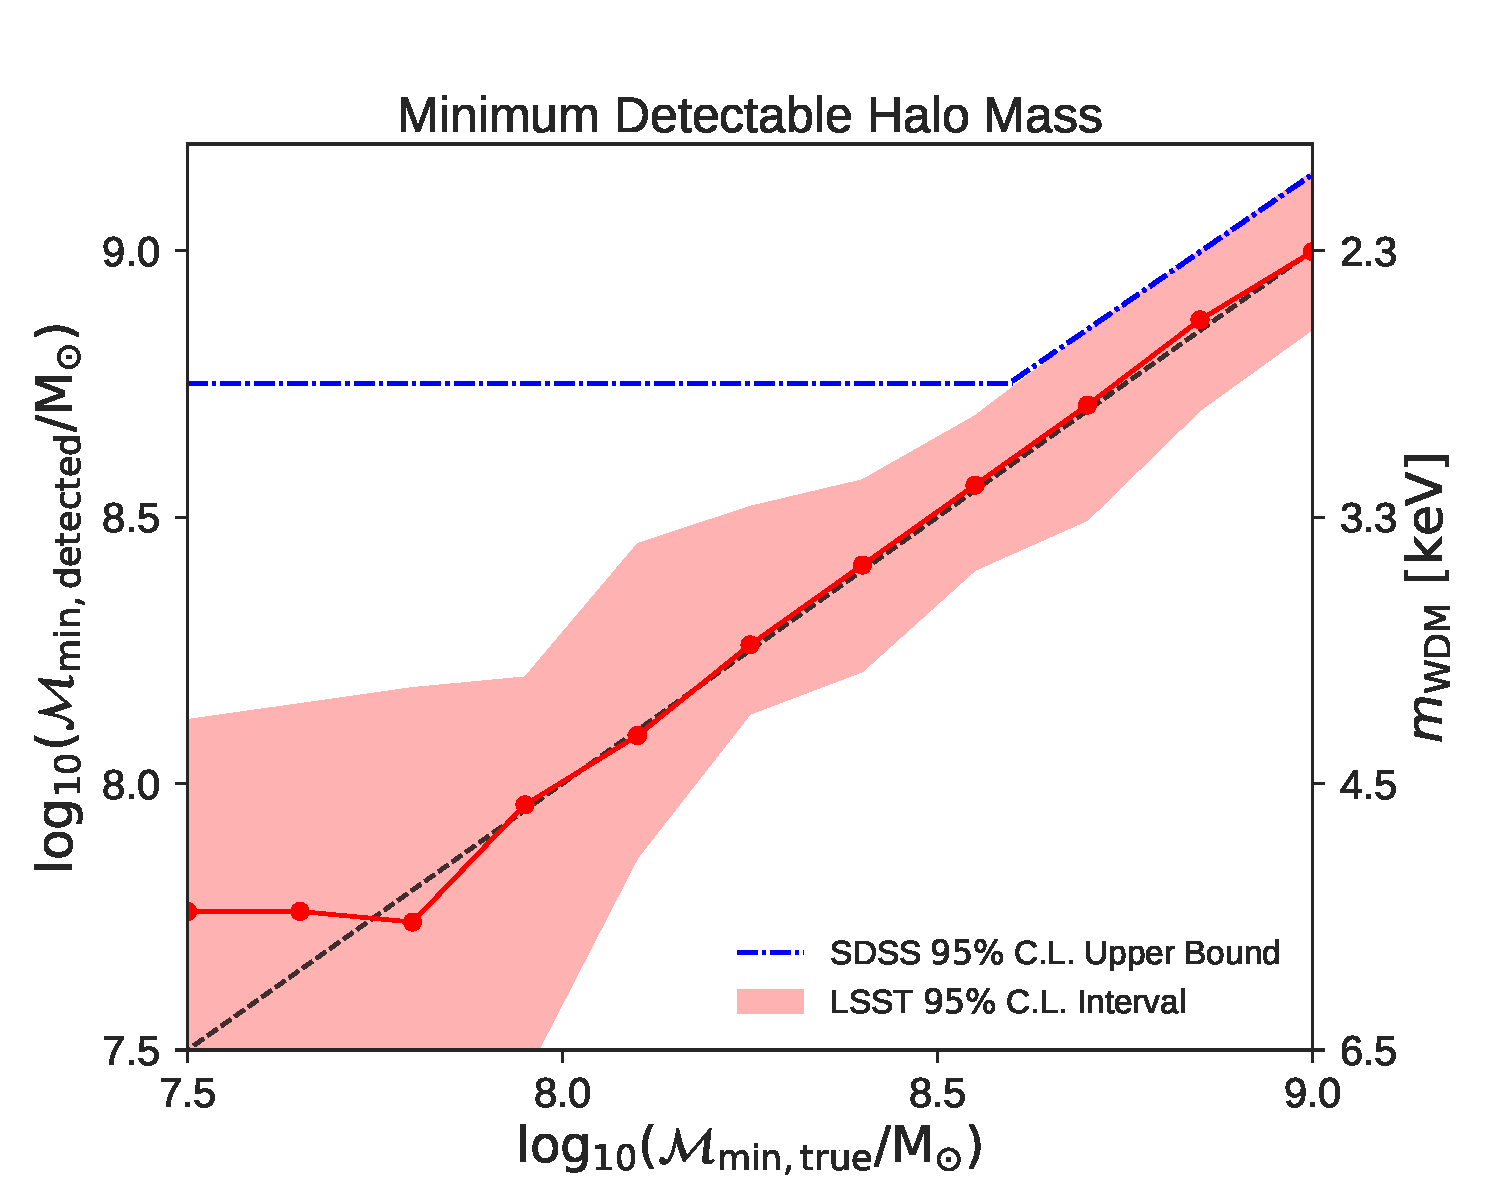
\includegraphics[width=0.775\textwidth]{figures/LSST_Mmin.pdf}
\caption{Forecast for the minimum dark matter subhalo mass probed by LSST via observations of Milky Way satellites. The red band shows the $95\%$ confidence interval from our MCMC fits to mock satellite populations as a function of the true peak subhalo mass necessary for galaxy formation. Note that we marginalize over the relevant nuisance parameters associated with the galaxy--halo connection---including the effects of baryons using a model calibrated on subhalo disruption in hydrodynamic simulations \citep{2018ApJ...859..129N}---in our sampling. We indicate the corresponding constraints on the warm dark matter mass assuming $M_{\rm hm} = \mathcal{M}_{\rm{min}}$ (see \secref{wdm})}\label{fig:satellite_mmin}
\end{figure}

The least luminous galaxies currently known contain only a few hundred stars and have been found exclusively in the inner regions of the Milky Way due to observational selection effects. Although the census of Milky Way dwarf galaxies has grown from $\roughly 25$ to more than 50 in recent years \citep[\eg, with DES;][]{Bechtol:2015, Koposov:2015, Drlica-Wagner:2015}, our current census is certainly incomplete.
For example, the HSC-SSP Collaboration has detected two ultra-faint galaxy candidates in the first $300 \deg^2$ of the survey \citep{1609.04346,1704.05977}; these galaxies are faint and distant enough to have been undetectable in previous optical imaging surveys. HSC is representative of the depth that will be achieved by LSST over half the sky---an area 60 times larger than the current HSC-SSP footprint. Thus, based on the results of SDSS, HSC, DES, etc., several groups have predicted that LSST could detect %at least 20 --- and as many as 50 \EON{check numbers} \ADW{Seems a bit small. I thought Hargis predicted $\roughly250$.} \AHGP{Check out the numbers from Table 1 of Kim, Peter, \& Hargis: we predict 50-600 depending mostly on the radial distribution of satellites in the halo.  The lower number is the most conservative choice, for a population of UFDs concentrated at the center of the halo, and is consistent with Newton et al.  The largest number is what we predict if the hydro sims of satellite disruption are correct.}--- 
tens to hundreds of new low-luminosity Milky Way satellites, mainly at larger distances and fainter luminosities than those accessible with current-generation surveys \citep{Koposov:2008,Tollerud:2008,Hargis:2014,Newton:2018,Jethwa:2018,Nadler:2018,Kim:2017iwr}. 
In addition, novel techniques, such as the use of the correlated phase space motions of stars \citep{1507.04353,1805.02588} or clustering of variable stars \citep{1507.00734} could further expand the sample of ultra-faint galaxies.
LSST observations of Milky Way satellites therefore offer an exciting testing ground for dark matter models; for example, the measured abundance, luminosity function, and radial distribution of Milky Way satellites \emph{already} place competitive constraints on warm dark matter particle mass at the level of 3--4\keV \citep[\eg,][]{Jethwa:2018,Kim:2017iwr}.%, and these constraints will improve as observations continue to probe the low-mass end of the subhalo mass function.

To relate these questions to LSST observations, we have analyzed simulated ultra-faint galaxies as they would appear in LSST WFD coadd object catalogs to quantify LSST's ability to detect nearby satellite galaxies. %, and we have developed a theoretical framework to connect observations of the Milky Way satellite population to the underlying dark matter subhalo population. 
We detect ultra-faint galaxies as arcminute-scale statistical overdensities of individually resolved stars; in ground-based optical imaging surveys, it is often challenging to classify low signal-to-noise catalog objects near the detection threshold as either foreground stars or unresolved background galaxies. LSST will reach depths at which the galaxy counts far outnumber stellar counts, so the search sensitivity for ultra-faint galaxies will largely be determined by our ability to accurately perform star-galaxy separation at magnitudes $24 < r < 27.5$; importantly, our sensitivity analyses include these effects. 
%In detail, we inject many simulated stellar populations into the center of the LSST DESC DC2 simulated data set and 
We find that Milky Way satellites within $300\kpc$ are well-detected with a surface brightness detection threshold of $\mu = 32\ \rm{mag\ arcsec}^{-2}$ \citep{0912.0201} and an absolute magnitude cutoff of $M_V = 0\magn$.

\figref{satellite_mmin} shows the minimum subhalo mass that LSST can probe via observations of Milky Way satellites, obtained by folding our search sensitivity estimates through a cosmological model of the Milky Wway satellite population that predicts satellite luminosity functions, radial distributions, and size distributions that agree well with current observations. In particular, we generate many mock Milky Way satellite populations using the model presented in \cite{Nadler:2018} given a ``true" value of the minimum peak subhalo virial mass necessary for galaxy formation, $\mathcal{M}_{\rm{min,true}}$, marginalizing over the remaining galaxy--halo connection parameters. We then perform mock observations of these generated satellite populations using the LSST selection function, and we compare these to the true satellite populations by MCMC sampling $\mathcal{M}_{\rm{min}}$ and the remaining galaxy--halo connection parameters assuming that satellite number counts are Poisson distributed in bins of absolute magnitude (see \citealt{Nadler:2018} for details on the fitting procedure). For each value of $\mathcal{M}_{\rm{min,true}}$, this procedure yields a posterior distribution over the minimum halo mass inferred by LSST observations. The red band in \figref{satellite_mmin} illustrates the recovered $95\%$ confidence interval as a function of $\mathcal{M}_{\rm{min,true}}$, and the blue dot-dashed line indicates the minimum halo mass inferred from known classical and SDSS-detected Milky Way satellites. 
%LSST observations recover the true minimum halo mass at large values of $\mathcal{M}_{\rm{min,true}}$, since all of the predicted satellites are observable in this regime, while smaller values of $\mathcal{M}_{\rm{min,true}}$ yield satellites that do not pass our detection criteria, which prevents the lowest-mass subhalos that host satellites to be detected. 
For small $\mathcal{M}_{\rm{min,true}}$, the $95\%$ confidence level upper bound on the lowest detectable subhalo mass improves by a factor of $\sim 5$ with LSST, from $\sim 5 \times 10^{8}\ \Msun$ to $\sim 10^{8}\ \Msun$; this translates to a lower bound of $\sim 7\ \rm{keV}$ on WDM particle mass (see \secref{combine_probes} for details).

Although we have presented a ``population-based'' forecast for dark matter constraints from LSST-detected ultra-faint satellites, we note that kinematic data obtained by follow-up spectroscopy of newly discovered satellites also offers a powerful probe of dark matter microphysics. We estimate the number of LSST-detected Milky Way satellites that can be spectroscopically confirmed in \secref{spectroscopy}, and we forecast the constraints offered by these stellar velocity dispersion measurements for WDM and SIDM in \secref{combine_probes}.

Further extending the sensitivity of LSST to a power spectrum cut-off on scales smaller than the mass threshold for galaxy formation requires techniques that are independent of satellite luminosity and that can detect subhalos purely through their gravitational signatures. Two examples of such probes are described in the following subsections.


\subsection{Stellar Stream Gaps \Contact{David H.}}
\label{sec:stream_gaps}
\Contributors{David Hendel, Nora Shipp, Ting S.\ Li, Ana Bonaca, Jo Bovy, Sergey Koposov, Denis Erkal, Nilanjan Banik, Andrew B.\ Pace}

Stellar streams, in particular the tidally disrupting remnants of globular clusters, are fragile, dynamically cold systems and are sensitive tracers of gravitational perturbations \citep[][]{2002MNRAS.332..915I,2002ApJ...570..656J,2011ApJ...731...58Y,Carlberg:2012}.
The main track of a stream in 6D phase space is shaped primarily by the Milky Way's global matter distribution while the detailed structure of the stream contains information about small-scale perturbations. 
In particular, a dark matter subhalo passing by the stream will provide a net velocity kick, altering the orbits of the closest stream stars.
The main observable consequence of this interaction is the formation of a gap in the density of stars along the stream; the relative depth and size of the underdensity can be used to infer the time since the encounter and the properties of the perturber \citep{Carlberg:2012, Erkal:2015}. The mass required to produce an observable gap \citep[$10^5$--$10^6 \Msun$,][]{erkal2016,bovy:2017} is well below the limit where dark matter subhalos are expected to host galaxies. Thus, stellar streams provide one of the most exciting near-field tests of the minimum subhalo mass.

Current constraints on the minimum subhalo mass from stream gaps are limited by the small number of streams that are bright enough that observations can detect density variations at a useful signal-to-noise ratio. Deep and precise LSST photometry is expected to increase the contrast between streams and the contaminating Milky Way field stars, to have improved star-galaxy separation, and to extend much farther down the color-magnitude diagram for known streams, dramatically increasing our ability to detect density variations and thus leading to the identification of less prominent gaps created by low-mass perturbers. Critically, with LSST we move from examining individual gaps into the regime where we can ask questions about subhalo population statistics and their (in)consistency with cold dark matter.
Here we estimate the least massive subhalo that can be detected with LSST observations of gaps in stellar streams.

We consider a mock-stream observed at a Galactic latitude of $b=-60^\circ$ in the $g$- and $r$-band. We assume the stream is old (12\,Gyr), metal-poor ($Z = 0.0002$), thin (1$\sigma$ stream width of 20\,pc), and cold (velocity dispersion of 1\,km\,s$^{-1}$) We generate synthetic photometry of the stream at a given mean surface brightness (within the $1\sigma$ width) and over a range of heliocentric distances from 10 to $40\kpc$.  Simulated stream stars are drawn from a Chabrier IMF \citep{2003PASP..115..763C}, while a synthetic background of Milky Way stars is generated from the \code{Galaxia} model \citep{sharma2011}. 
We add noise to the simulated photometric measurements for both the stream and Milky Way stars in accordance with expectations for LSST \citep{0805.2366}. 
We then select stars in the color-magnitude diagram that are within $2\sigma$ of the theoretical isochrone of the stream's age and metallicity, where $\sigma$ is the magnitude-dependent photometric uncertainty using the same error model. 
% we assume $\sigma$ is no less then 0.02 mag (i.e. set to 0.02 if it's smaller).
We also assume a limiting magnitude to set the depth of the survey, choosing the point where the photometric uncertainty in either band exceeds 0.1 mag. We apply this color-magnitude selection to determine the density of stream stars and background stars.
The depth of the gap from a given subhalo mass is calculated using the theoretical relation derived by \citet{erkal2016}, assuming that the subhalo impact occurred within the past $0.5\Gyr$, moving at $150\kms$, with an impact parameter equal to the perturber's scale radius. Finally, we define a detection as a gap depth that is $5\,\sigma$ above the noise background (the effects of star-galaxy separation are not considered in this calculation).

\begin{figure}[t]
\centering
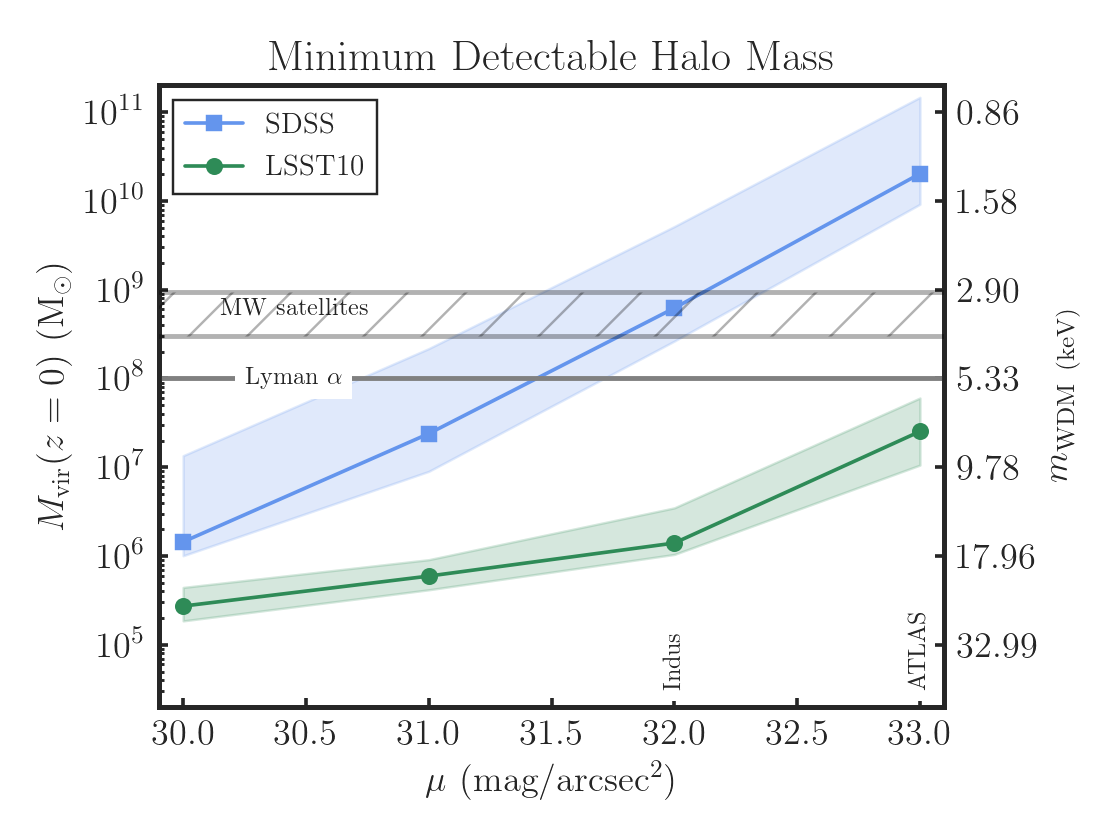
\includegraphics[width=0.85\textwidth]{figures/streamgap_constraints_3.png}
\caption{\label{fig:streamsurveys} Detection limits for gaps formed from subhalos of different masses using photometry from SDSS (blue) or the 10-year LSST stack (green) as a function of the stream surface brightness.
Shaded regions correspond to a 10-40 kpc distance range, with the lines representing 20 kpc. For streams with surface brightnesses similar to those found in DES, 32--$33 \magn \asec^{-2}$, LSST is expected to probe halo masses two to three orders of magnitude smaller than SDSS and substantially improve the current constraints from Milky Way satellites \citep{Nadler:2018, Jethwa:2018,Kim:2017iwr} and the Lyman-$\alpha$ forest \citep{2017PhRvD..96b3522I}. 
We connect the detected halos to the mass of the warm dark matter particle that would produce a minimum halo of that mass using the relationship determined by \cite{Bullock:2017}. Note that the halo mass definition used here is the $z=0$ virial mass; to relate this quantity to the peak subhalo mass used in our warm dark matter constraints, we have assumed the best-case scenario of no tidal mass loss.
}
\end{figure}


\figref{streamsurveys} shows the lowest-mass dark matter subhalo detectable using the 10-year LSST data as a function of stream surface brightness and heliocentric distance. For a stream with a surface brightness of 33 (31.5) $\mathrm{mag}\,\mathrm{arcsec}^{-2}$, LSST is able to detect subhalos with $M_{\rm vir}(z=0) \sim 2 \times 10^7 \Msun$ ($1 \times 10^6 \Msun$) at 20 kpc.
%\footnote{Note that these correspond to $z=0$ virial masses; to convert these into the peak mass that enters our half-mode mass estimate, we measure the mean $M_{\rm{peak}}$--$M_{\rm{vir}}$ relation from the highest-resolution simulation presented in \cite{Mao2015}.} 
As a comparison, we used the same model to calculate the gap detectability using SDSS DR9 photometry. LSST provides $\roughly 3$ orders of magnitude improvement at low surface brightnesses, where most known (and anticipated) streams lie. Crucially, this pushes the minimum detectable halo mass below current constraints from Milky Way satellites \citep[\eg,][]{Nadler:2018,Jethwa:2018,Kim:2017iwr} or the Lyman-$\alpha$ forest \citep[\eg,][]{2017PhRvD..96b3522I}.
To set constraints on \Mhm and \mWDM, we convert $M_{\rm vir}(z=0)$ to $M_{\rm peak}$ using a relation derived from the highest-resolution simulation presented in \citet{Mao2015}.\footnote{We find a mean relationship of: $\log_{10}(M_{\rm peak}) = 0.88 \log_{10}(M_{\rm vir}) + 1.28$.}
We then follow the same formalism as in \secref{smallest_galaxies} to convert from $M_{\rm peak}$ to $\Mhm$ and calculate \mWDM from \eqnref{mWDM}.


Given a gap density detection threshold and a subhalo population, this formalism can be used to predict the number of gaps in a given stream \citep{erkal2016}. Typically, this predicts $\roughly 1$ gap per stream, making it difficult to interpret well-studied individual streams (i.e. Palomar 5 and GD-1). LSST is expected to measure dozens of streams as precisely as Palomar 5 and GD-1 have currently been mapped and will therefore provide a much stronger constraint: at the 10-year LSST depth, \LCDM predicts that we should observe 17 gaps total in the 13 DES streams reported by \cite{2018ApJ...862..114S}. Observing fewer than 6 gaps would be inconsistent with \LCDM at a 99.9\,\% level. 

A single stellar stream is expected to experience several subhalo encounters over its dynamical lifetime. 
Recent strong impacts will result in the observable gaps described above, while weaker encounters will cause less prominent density and track variations.
The effects of ancient impacts will be gradually erased due to the internal velocity dispersion of the stream member stars; however, it is possible to extract statistical information about the impact history of the stream by studying the linear density and track power spectra, both of which are sensitive to the subhalo mass functions.
Impacts from higher-mass subhalos introduce power on large scales, while lower-mass subhalo impacts introduce power on small scales. 
Statistical analyses of the stream density power spectrum have been used to constrain the number of subhalos within the stream radius and the properties of dark matter \citep{bovy:2017, 2018JCAP...07..061B}. 
LSST will allow us to measure the stream density and stream track power spectra at small angular scales that were previously dominated by noise, and \citet{bovy:2017} project that the power spectrum method will be sensitive to subhalos down to mass $10^5 \Msun$. 
In addition, precise measurement of the densities and tracks of multiple streams can be combine to increase statistical power and mitigate systematics from any individual stream.


Depending on their orbits, stellar streams can also be perturbed by the baryonic structures such as the Galactic bar \citep[\eg,][]{erkal2017,pearson2017}, spiral arms \citep{Banik2018}, or giant molecular clouds \citep{amorisco2016}. The resulting gaps may be difficult to distinguish from gaps induced by dark matter subhalos and can bias measurements toward overestimating the number of subhalo impacts on a stellar stream. The only recourse is to carefully examine the streams' orbits to assess these possible confounding factors. Streams with pericenters of $\gtrsim 14\kpc$ should be relatively unaffected by these baryonic factors, and streams on retrograde orbits even less so. In addition, subhalos may also experience extra tidal shocks from the disk, which can alter the number of expected impacts in a given cosmological model \citep[\eg,][]{DOnghia:2009xhq,Garrison-Kimmel2017}. LSST will mitigate both of these issues by examining streams farther from the center of the Galaxy where these effects are lessened.

In this summary we have only considered the density structure of the stream. However, the perturbation that creates the gap necessarily affects the other phase space dimensions as well. The inclusion of these phase space dimensions allows for an almost unique determination of both the subhalo's internal and impact properties for each gap \citep{erkal2015b}. Furthermore, the perturber's effect produces a correlated signal across observables, improving the precision with which the statistical properties of the stream (\eg, power spectrum and cross-correlation of observables) can be used to measure subhalo properties \citep{bovy:2017}. This provides an exciting opportunity for synergy with current and future spectroscopic and astrometric surveys in addition to precise photometric distances and proper motions from LSST itself. Such efforts will greatly aid in the removal of foreground and background contamination, and they will tighten constraints on the stream progenitor's orbit and provide better measurements of the perturber's mass and size. See \secref{complementarity} for a discussion of some complementary science programs.

\subsection{Strong Lensing \Contact{Chris F.} }
\label{sec:stronglens} 
\Contributors{Christopher D.\ Fassnacht, Cora Dvorkin, Francis-Yan Cyr-Racine, Charles R.\ Keeton, Yashar D.\ Hezaveh, Ana~D\'{i}az Rivero}

Strong gravitational lensing is one of the most powerful probes of dark matter halos beyond the Local Goup. 
Gravitational lensing directly probes the total mass distribution that a light ray encounters and does not require that mass to be luminous or baryonic.
Therefore, an analysis of lensing signals can be used to measure the presence, quantity, and mass of subhalos in massive galaxies and small isolated halos along the line-of-sight.  
The discovery of low-mass dark matter halos is possible even at cosmological distances, where the flux of any luminous material associated with the halos would fall below the detection limits of typical observations.  
Thus, the gravitational lensing approach is highly complementary to Local Group observations.

The (sub)halo-detection techniques described below utilize strong gravitational lensing, in which a massive foreground object bends the light from a background galaxy to produce multiple images of the background object.  
If the emission from the background object is dominated by a single point-like component, such as a quasar or other AGN, the lens system will contain multiple images of that component (\eg, \figref{stronglens_examples}a).
Typically these quasar lens systems consist of two or four images, creating ``doubles'' and ''quads'' respectively. 
If, on the other hand, the background object is dominated by stellar emission, then the lensed emission is in the form of tangentially stretched arcs or a full Einstein ring that surrounds the lensing galaxy (\eg, \figref{stronglens_examples}b).  
In both cases, substructure in the main lensing galaxy and small line-of-sight halos create small perturbations to the lensed images.

As will be described in detail below, there are three main techniques for detecting the presence of dark (sub)halos using strongly lensed systems: analysis of flux-ratio anomalies in lensed quasar systems,
gravitational imaging for lensed galaxy systems, and power spectrum approaches. 
Improved constraints on dark matter properties via these measurements will require: (1) a much larger samples of lens systems, and (2) follow-up observations with high-resolution imaging and spectroscopy.
LSST will play a critical role by increasing the number of lensed systems from the current sample of hundreds to an expected samples of thousands of lensed quasars \citep{O+M10} and tens of thousands of lensed galaxies \citep{Collett2015}.
The vast increases in sample sizes will provide much stronger statistical constraints on dark matter models than are currently possible (\eg, \figref{lensing_wdmlim_vs_nlens}).
The study of lensed systems will also require coordination with other facilities, namely space-based observatories, large ground-based telescopes with adaptive optics systems, ALMA, and very-long-baseline radio interferometry (see \secref{SLcomplement}). These facilities provide the milliarcsecond-scale angular resolution that is required to push the (sub)halo detection sensitivity into unexplored mass regimes.

\begin{figure}
    \centering
    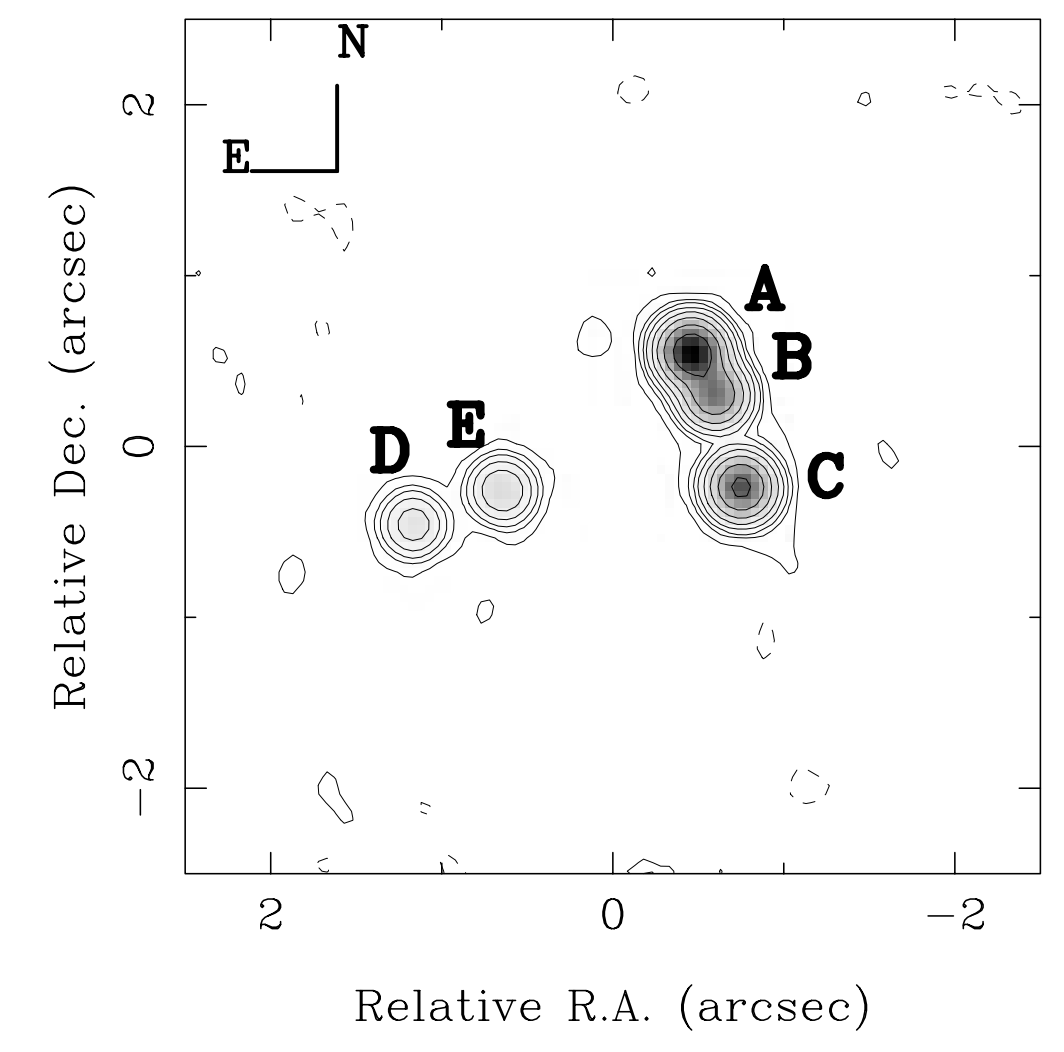
\includegraphics[width=0.4\textwidth]{2045_vla_dec96_x.png}    
    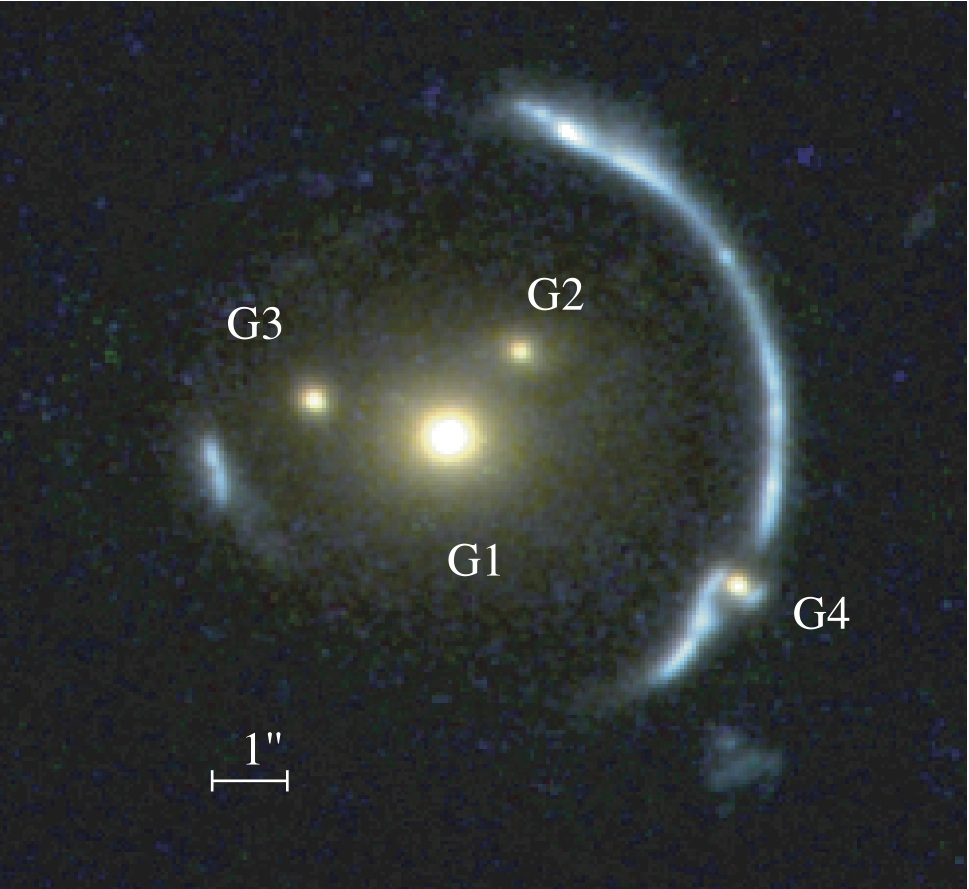
\includegraphics[width=0.44\textwidth]{Clone_labeled.png}
    \caption{Examples of two gravitational lens systems that exhibit perturbations due to (potentially unseen) halos.  {\bf (a)} Radio-wavelength imaging of a quasar lens system, B2045, that has one of the strongest flux-ratio anomalies known.  Component B should be the brightest of the three close images and instead it is the faintest. Figure from \citet{Fassnacht++99}
    {\bf (b)} HST imaging of the ``Clone'' \citep{2009ApJ...699.1242L}, showing that the long lensed arc is split by the presence of a perturber, in this case galaxy G4.  Note that the location and mass of G4 could have been determined {\em even if G4 were purely dark}.  Figure from \citet{Vegetti_2010_1}.}
    \label{fig:stronglens_examples}
\end{figure}

\begin{figure}
    \centering
    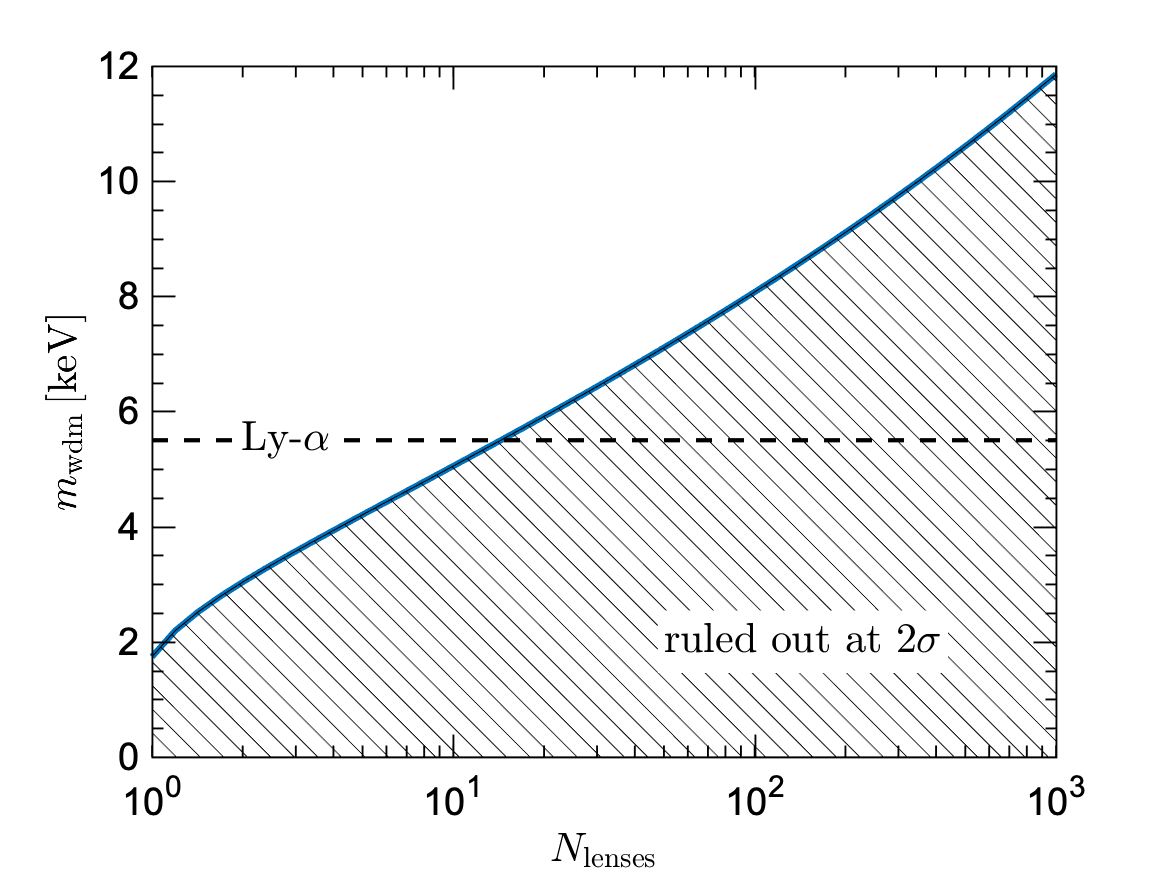
\includegraphics[width=0.70\textwidth]{wdm_constraints_yh.png}
    \caption{ \label{fig:lensing_wdmlim_vs_nlens} Projected $2\sigma$ constraints on WDM particle mass as a function of the number of strong lens systems that achieve a given (sub)halo mass detection threshold, under the assumption that CDM is correct. These constraints include only the contribution from halo substructure, and do not include the line-of-sight contribution.
Exisiting Lyman-$\alpha$ forest constraints are shown with a dashed horizontal line \citep{2017PhRvD..96b3522I}. Figure based on \citet{Hezaveh_2016ltk}.
}
\end{figure}


\vspace{1em} \noindent {\bf Flux-ratio Anomalies}

The presence of clumpy (dark) matter, whether within the main halo of the primary lens or along the line of sight, will perturb the gravitational potential of a strong lens system.
One of the effects of these perturbations is to change the magnification of the lensed images of a background AGN.
The angular scales over which the perturbations are important depend on the mass the perturber, so the presence of a small (sub)halo will typically affect only one of the lensed images and, thus, will change the relative fluxes of the images.
Furthermore, because the image magnification depends on the second derivatives of the gravitational potential, this method is, in theory, sensitive to smaller-mass structures than the gravitational imaging approach described below.\footnote{Indeed, flux-ratio anomalies can be produced by stars in the lens galaxy, through the microlensing phenomenon discussed below.}

The utility of this effect was first presented in \citet{Mao:1998aa}, which considered the effects of spiral arms in the lensing galaxy on the flux ratios of the lensed images, and for many years this was the only lensing technique used to investigate the presence of substructure in massive galaxies.
The approach is to describe the lensing galaxy with a relatively simple smooth single halo model.
These simple models are nearly always capable of fitting the observed positions of the lensed images to within the observational errors.
At that point, any deviation between the model-predicted image fluxes and the observed fluxes could be ascribed to some type of non-smooth / clumpy mass, either in the lensing galaxy or along the line of sight.
At optical and near-IR wavelengths, there are often significant differences between the predicted and observed image fluxes.
However, these perturbations are most likely to be produced by stars in the lensing galaxies, a process known as microlensing, and thus optical and near-IR fluxes are not informative in terms of the statistics of dark matter halos.
What is required is to observe at wavelengths at which the angular size of the emitting region in the background source is large compared to the micro-arcsecond scales at which stars produce their effects.  
Until recently, this meant observing lensed quasar systems at radio or mid-IR wavelengths, which vastly reduced the available sample sizes.

A seminal paper by \cite{Dalal:2002aa} used the statistics of observed flux-ratios in a sample of seven lens systems to place limits on the substructure fraction in the lensing galaxies, i.e., the percentage of the lens mass that is composed of clumpy structures, in the $10^6 - 10^9 \Msun$ range.
The small sample size was set by the number of radio-loud systems that was known at the time and the one lens system with a usable mid-IR data set.  
Because lensed radio-loud AGN are rare, and ground-based high-resolution mid-IR observations are extremely difficult, the sample size only increased by a few lenses over the next decade.  
Forecasts based on forward modeling simulations indicate that $\gtrsim$100 well-constrained flux-ratio systems are needed to provide 2$\sigma$ constraints of $10^{7.2} - 10^{7.5} \Msun$ for the half-mode mass in a WDM scenario, corresponding to a $\sim$5--6~keV thermal relic mass \citep{Gilman++18}.
More recent estimates including line-of-sight structure show that similar constraints may be achievable with $\roughly 50$ lenses \citep{1901.11031}.
In either case, increases in sample sizes are required.
The two most promising paths forward are to obtain large lensed quasar samples with LSST and then follow up with either high-resolution mid-IR imaging with JWST, or IFU spectrographs on ELTs or JWST.  The second technique takes advantage of the fact that in lensed AGN, the narrow-line region surrounding the central AGN is larger than the microlensing scale, even though the broad-line region and the source of the continuum emission are not.  Therefore, with high-resolution IFU observations, the narrow-line emission from each lensed image can be spatially resolved, thus providing the required microlensing-free flux ratios \citep{MoustakasMetcalf03, Nierenberg++14, Nierenberg:2017vlg}.

Deep high-resolution imaging in the optical or infrared is also necessary to address possible systematics in the flux-ratio technique.  
Investigations using Keck adaptive optics imaging of radio loud lenses have shown that, in some cases, the observed flux-ratio anomalies can be explained by baryonic structures in the lensing galaxy, namely edge-on stellar disks rather than dark matter halos \citep{Hsueh++2016, Hsueh++2017}.
These baryonic effects were also seen in simulated data \citep{Gilman++2017, Hsueh++2018}.
These studies indicate that a lack of knowledge about the baryonic structure of the lensing galaxy may lead to an overestimate of the amount of clumpy dark matter in the lens or along the line of sight.
With a sample of thousands of quasar lenses expected from LSST, it will be possible to select systems where baryonic effects are minimized.

\vspace{1em} \noindent {\bf Gravitational Imaging}

The presence of a massive peturber along the line of sight can change the shape of lensed emission. 
This effect can be utilized in strong lens system in which the background object is a galaxy that is lensed into long arcs or a complete Einstein ring.
Small (sub)halos that are close in projection to the lensed emission can distort arc shape to a degree that can be detected by high-resolution imaging observations.
This ``gravitational imaging'' technique was proposed by \cite{Koopmans:aa} and further refined by \citet{Vegetti:2008aa,Vegetti:2009aa}.  The size of this effect depends on the mass of the perturber and its projected distance from the lensed arcs, with more massive and closer perturbers having larger effects.
 
The first application of the gravitational imaging technique to real data was for the ``Clone,'' a system for which the primary lensing halo is a compact galaxy group \citep[\figref{stronglens_examples},][]{2009ApJ...699.1242L, Vegetti_2010_1}. In this system, the long lensed arc is broken and split at the location of the peturber, which in this case is a satellite galaxy in the group with a mass of $\roughly 10^{10} \Msun$ \citep[][]{Vegetti_2010_1}.  This massive galaxy located right on the arc produced an effect that could be seen by eye in high-resolution HST imaging.  Lower-mass detections were subsequently made using HST \citep[$\roughly 10^9 \Msun$;][]{Vegetti_2010_2}, Keck adaptive optics \citep[$\roughly 10^8 \Msun$;][]{Vegetti_2012}, and ALMA mm-wave interferometry \citep[$\roughly 10^8 \Msun$;][]{Hezaveh_2016ltk}.  
Note that the masses reported in these papers usually assume a truncated mass distribution (\eg, a pseudo-Jaffe profile) or are explicitly given as mass contained within radii of, \eg, 600\pc, to better match dwarf galaxy measurements made within the Local Group.  Multiplying these values by a factor of 10 gives roughly the expected virial mass of their host halos.
 
The implications for the nature of dark matter from the gravitational imaging technique come from comparing the number of detected halos to those predicted by various dark-matter models.  
For this reason, one of the strengths of the technique is that {\em non-detections} are as valuable as detections, and can be especially powerful at low masses where CDM models predict a large number of halos.
This analysis relies on an understanding of the lowest mass that can be detected at each location in the lens system \citep[\eg,][]{Vegetti2014, Hezaveh_2016ltk, Ritondale++18}.
 
Nearly all previous inferences on dark matter from gravitational imaging have considered solely the expected and measured effects of subhalos within the main halo of the primary lensing galaxy \citep[\eg,][]{Vegetti:2009aa, Vegetti_2012, Vegetti2014, Hezaveh_2016ltk}.
However, an additional perturbation signal is provided by the presence of halos along the line of sight.
An analysis of simulated data has shown that the signal from line-of-sight structures is significant even for lower redshift lenses and is the dominant contribution to any lensing signal for higher redshifts \citep{Keeton:2002ug,Despali++18}.
The line-of-sight structures may very well be a cleaner probe of dark-matter properties than substructures in the lensing galaxies.
This is because the line-of-sight halos are unlikely to have been tidally stripped and thus their measured masses reflect their true masses.
The techniques for including the line-of-sight signal have been developed and applied to recent analyses \citep{Ritondale++18}. 
 
For the relatively high (sub)halo masses that have been probed so far, $\gtrsim 10^9\Msun$, there is little difference between the predictions of CDM and models with a mass cutoff (\eg, WDM).
Therefore, even analyses of $\roughly10$-lens samples have not achieved the statistical precision to distinguish between dark matter models \citep{Vegetti2014, Ritondale++18}.
What is urgently needed is both to increase the sample sizes and, more importantly, to probe further down the mass function.
The mass-detection limit for gravitational imaging is set by three properties of the observations: (1) the signal-to-noise ratio, (2) the angular resolution of the imaging data, and (3) the surface-brightness structure of the lensed background galaxy.  This last point arises because it is easier to detect small astrometric shifts if there are strong gradients in the surface brightness, as opposed to a smooth light distribution.
These properties lead to the need for sensitive high resolution observations of the large samples of appropriate lenses that LSST will provide.
The high-resolutions observations can come from ELTs, which should provide milliarcsecond-scale angular resolution currently only available from VLBI radio observations.
For the subset of LSST lenses that are radio loud, VLBI and ALMA observations will provide excellent complementarity.

\vspace{1em} \noindent {\bf Small-scale Structure Power Spectrum}
\begin{figure}[t]
\centering
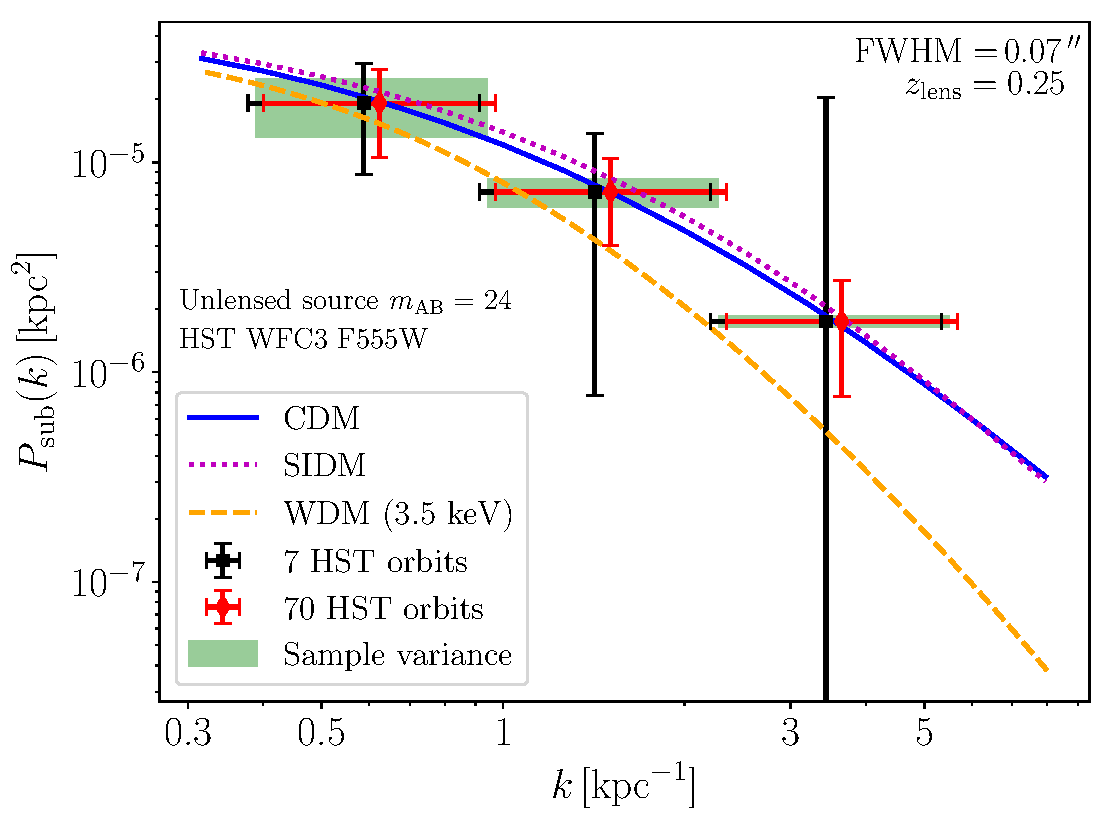
\includegraphics[width=0.6\textwidth]{Fisher_space_Pk_SIDM_rev.pdf}
\caption{Fisher forecast for the substructure convergence power spectrum in three logarithmic wavenumber bins. We consider here observations with the wide-field camera 3 (WFC3) aboard the Hubble Space Telescope (HST) using the F555W filter, resulting in a point-spread function FWHM of $0.07$ arcsec. The source is placed at $z_{\rm src}=0.6$ with an unlensed magnitude $m_{\rm AB}=24$. The error bars show the $1$-$\sigma$ regions, while the green rectangles display the sample variance contribution within each bin. We conservatively assume that only half of each orbit is available for observation. The blue solid line shows the fiducial substructure power spectrum model used in the forecast, which corresponds to a CDM population of subhalos modeled with truncated NFW profiles. The dotted magenta line shows the power spectrum for SIDM, assuming a subhalo core size equals to $70\%$ of the scale radius. For comparison, the orange dashed line shows the substructure power spectrum for a thermal relic warm DM with mass of 3.5 keV \citep{Viel:2013}. Figure adapted from \cite{Cyr-Racine:2018htu}. \label{fig:pksub_fisher}}
\end{figure}

While gravitational imaging can detect highly significant and well-localized perturbers along lensed arcs and Einstein rings, less massive perturbers or those located farther away from lensed images typically lead to observational signatures that are too subtle to be detected individually. However, the large number of such perturbers, both as subhalos within the lens galaxy and as field halos along the line of sight, means that their collective effect might be detectable at the statistical level \citep[\eg,][]{Birrer2017}. The power spectrum of the lensed deflection field is a particularly powerful quantity for capturing the aggregate behavior of lensing perturbers. This approach was proposed in \cite{Hezaveh_2014}, and further expanded in \cite{Rivero:2017mao}, \cite{Chatterjee_2017}, and \cite{Cyr-Racine:2018htu}. 
Furthermore, \cite{Daylan:2017kfh} proposed a technique to constrain the statistical properties of dark matter subhalos in the lens galaxies by studying the joint perturbations of unresolved subhalos.

A key advantage of this power spectrum approach is that it describe the effect of perturbers in terms of a \emph{spatial fluctuation} basis instead of the more traditionally used \emph{mass} basis. The power spectrum directly captures the spatial scales on which perturbers influence the lensed images without having to invoke the notion of (sub)halo density profile, the latter of which is usually required to map from the perturber mass space to the resulting spatial deflection field. As such, the power spectrum is a natural language to describe the collective effects of small lensing perturbers. 

To develop intuition about which dark matter properties could be probed from measurement of this new lensing statistic, \cite{Rivero:2017mao} developed a general formalism to compute from first principles the convergence power spectrum for different populations of subhalos (not yet including line-of-sight perturbers). The authors pointed out that this power spectrum can be mainly described by three quantities: a low-wavenumber amplitude, that depends on the subhalo abundance and on specific statistical moments of the subhalo mass function; on a turnover scale, that probes the truncation radius of the largest subhalos in the system; and on a higher-wavenumber ($k\gtrsim 1 \kpc^{-1}$) slope, that probes a combination of the subhalo inner density profiles and of a possible cutoff in the primordial matter power spectrum. These theoretical findings were then confirmed numerically in \cite{Brennan:2018jhq} using a semi-analytic galaxy formation model, and in \cite{Rivero:2018bcd} using high-resolution $N$-body simulations. Measurements of the power spectrum promise a wealth of information about the behavior of dark matter on small scales.

Several challenges need to be addressed to fully enable the constraining abilities of power spectrum measurements. Most importantly, the degeneracy between the possibly complex brightness profile of the source and the statistical effects of the lensing perturbers needs to be accurately explored. Also, the importance of line-of-sight structure remains to be properly quantified, and the effect of lens galaxy light and other luminous foregrounds on the power spectrum inference needs to be better understood. Finally, since instrumental artifacts such as a mismodeled point-spread function or camera sensitivity could potentially mimic a power spectrum signal, it is likely that these effects would have to be reconstructed at a higher precision than what is typically done for gravitational imaging. 

Thus far, measurement of the lensing power spectrum has been attempted by \cite{Bayer:2018vhy}, and an upper limit on its amplitude was derived using HST archival data. The currently known samples of galaxy-galaxy lenses numbers in the few dozens, and LSST is expected to increase this number several-fold as mentioned above. High-resolution follow up using either space-based or AO-enabled ground-based observatories will be required to measure the power spectrum from these targets and thus probe small-scale structure in a new way (\secref{SLcomplement}). \citet{Cyr-Racine:2018htu} has performed detailed forecasts for the sensitivity of different observational scenarios to the perturber power spectrum for lenses of the type that LSST is expected to discover at optical wavelengths (\figref{pksub_fisher}). It was found that images only a factor of a few deeper than what is currently typically available \citep[\eg, from the SLACS sample][]{Bolton2008} could be sufficient to detect the overall amplitude of the lensing power spectrum. On the other hand, constraining the slope at larger wavenumbers, which could help distinguish between WDM and CDM (\figref{pksub_fisher}), would require much deeper imaging.

\subsection{Satellite Joint Analysis  \Contact{Francis-Yan} }
%Minimum Halo Mass and Density Profile Measurements: 
\label{sec:combine_probes} 
\Contributors{Francis-Yan Cyr-Racine, Ethan O.\ Nadler, Manoj Kaplinghat, Alex Drlica-Wagner, Arka Banerjee, Kimberly K.\ Boddy}
 
As stated above, a cut-off in the matter power spectrum is related to early universe kinematics of dark matter particles and interactions of dark matter particles with a relativistic species. This cut-off directly affects both the subhalo mass function and the luminosity function of Milky Way satellites. Importantly, it also affects the internal properties of subhalos with masses near this threshold. Indeed, the power spectrum cut-off delays halo formation on mass scales near to and smaller than the cut-off, hence lowering the concentration of these objects at fixed halo mass \citep[\eg,][]{Dunstan:2011bq}. Since SIDM (\secref{sidm}) can also have a large impact on the central densities of small halos, combining information from minimum halo mass and density profile measurements (\secref{profiles}) can jointly constrain the presence of a cut-off and of a non-vanishing $\sigma_{\rm SIDM}$, hence simultaneously probing the cold and collisionless tenets of the CDM paradigm. As an illustrative example, we estimate the potential sensitivity of an analysis combining kinematic measurements of LSST-discovered Milky Way satellites with the minimum halo mass forecasts shown in \figref{satellite_mmin}. While not discussed here, we note that both stellar stream gaps and strong lensing could also be used for such joint analysis since they in principle have some sensitivity to internal properties of small halos as well. 

%\vspace{1em} \noindent {\bf Joint impact of a cut-off and self-interaction on the central densities of satellites}
\vspace{1em} \noindent {\bf Joint impacts on the central densities of satellites}

As a demonstration of the power of LSST to probe both a power spectrum cut-off and dark matter self-interaction, we focus here on a simplified summary statistic which captures the essence of LSST's constraining power. The reader should keep in mind that a more detailed analysis using the full complexity of the LSST data set (and its spectroscopic follow-up) could unveil even more information about dark matter physics. Specifically, we consider here the impact of self-interaction or a cut-off on the cumulative number of satellites above a given luminosity threshold that have stellar velocity dispersion within their half-light radius above a minimum value $\sigma_{\star,\rm lim}$, $N_{\rm sat}(L_\star>L_{\rm lim}, \sigma_\star> \sigma_{\star,\rm lim})$. Here, we use the stellar velocity dispersion, $\sigma_\star$, as a probe of the subhalo's central density.

%We model the connection between the central density of subhalos and the self-interaction cross section or cut-off in the power spectrum in the following way. 
For simplicity, we parameterize the cut-off in the power spectrum using the thermal WDM mass, $\mWDM$ \citep[\eg,][]{Bode:2000gq}, but note that other physics such as interactions with a relativistic species \citep[\eg,][]{Boehm:2004th,Cyr-Racine:2015ihg} could also cause a small-scale suppression of power. It is well-known that dark matter self-interaction creates constant density cores in the subhalos \citep{Spergel:1999mh}, which usually lowers the central density as compared to NFW halos. In the limit of large cross sections or significant subhalo mass loss, the self-interactions could also lead to core collapse and an increase in the subhalo central density \citep{Balberg:2002ue,Ahn:2004xt,Nishikawa:2019lsc}. 

In the absence of significant self-interaction, the power spectrum cut-off affects the central density through a modification of the subhalo concentration-mass relation \citep{Dunstan:2011bq,schneider2012,Lovell:2013ola,Bose:2016irl}. We adopt the following form for this modification  
\begin{equation}
c(M_{\rm vir}; \mWDM) = c_{\rm CDM}(M_{\rm vir})\left(\frac{M_{\rm vir}}{10^{12} \Msun} \right)^{\Delta\alpha(\mWDM)}\,,
\end{equation}
where $M_{\rm vir}$ is the subhalo virial mass, $c_{\rm CDM}$ is the subhalo concentration in the standard CDM case \citep{Moline:2016pbm}, and $\Delta\alpha$ is a power-law index that depends on the power spectrum cut-off. In this small self-interaction cross section limit, we assume that the core size is negligible and the density profile is of the NFW form. Note that stellar feedback can change this situation, a manifestation of the well-known degeneracy between feedback and self-interactions \citep[\eg][]{1996MNRAS.283L..72N}. 

In the opposite limit of large cores created by self-interactions, the central density $\rho_0$ of the subhalo can be written as \citep{Nishikawa:2019lsc}
\begin{equation}
\rho_0=\rho_{\rm s} f(t/t_0)\,,
\end{equation}
where $t$ is time elapsed since infall, $t_0 = a(\sigmam)\rho_{\rm s} v_0$ with $v_0^2=4\pi G \rho_{\rm s} r_{\rm s}^2$ and $a=\sqrt{16/\pi}$ for a hard-sphere interaction~\citep{Balberg:2002ue}. Here, $\rho_{\rm s}$ and $r_{\rm s}$ are the NFW density and scale radius parameters, respectively. The function $f$ encodes the evolution in time of the subhalo's central density in the presence of self-interactions, which includes its initial suppression due to core formation, and its subsequent increase due to the onset of the gravo-thermal instability \citep{Ahn:2004xt}. Importantly, the onset of this latter phase depends on the satellite's orbital history, with highly tidally stripped subhalos reaching it on a much shorter timescale than field halos \citep{Nishikawa:2019lsc}. To incorporate these results we make the further assumption that the tidal evolution of subhalos is not highly sensitive to dark matter particle physics. Current simulations tend to support this point of view, although it is likely that the stripped mass fraction will be somewhat larger for subhalos that have lower central densities due to either a cut-off in the power spectrum or self-interactions \citep{Lovell:2013ola,Dooley:2016ajo}. 

We adopt the following simple model for relating the mean stellar dispersion $\bar{\sigma}_\star$ to the central density $\rho_0$ \citep{Wolf:2009tu}
\begin{equation}
\bar{\sigma}_\star = 1 \kms \sqrt{\frac{\rho_0}{0.1 \Msun/{\rm pc}^3}} \left ( \frac{R_{\rm h}}{50 {\rm pc}} \right ) \,,
\end{equation}
which is valid as long as the core radius $r_{\rm c}$ is much larger than the projected half-light radius $R_{\rm h}$. In the opposite case where $r_{\rm c} < R_{\rm h}$, we modify this relation by putting an upper bound on $f(t/t_0)$ at a value given by $1/(x_{\rm h}(1+x_{\rm h})^2)$, where $x_{\rm h} = R_{\rm h}/r_{\rm s}$, and where the core radius is defined by the equation $\rho_{\rm NFW}(r_{\rm c}) = \rho_0$.   

To map the present-day mass of our subhalos to their luminosities, we combine the zoom-in simulations presented in \cite{Mao2015} with the subhalo--satellite galaxy model presented in \cite{Nadler:2018} to obtain the probability that a subhalo of present-day virial mass $M_{\rm{vir}}$ hosts a satellite of luminosity $L_\star$ and stellar dispersion $\sigma_\star$. The mapping from subhalos to satellites includes a prescription for hydrodynamic effects such as enhanced subhalo disruption due to a galactic disk, the galaxy formation threshold due to reionization, and a flexible model for the relationship between luminosity and subhalo peak circular velocity. To characterize $P(L_\star|M_{\rm{vir}})$, we sample from the posterior distribution of model parameters from the fit to classical and SDSS-detected satellites in \cite{Nadler:2018}, generate a large number of satellite population realizations for each Milky Way host halo, and fit the resulting $P(L_\star|M_{\rm{vir}})$ relation with a log-normal distribution. We also use these simulated satellite populations to perform a large number of mock LSST observations to obtain the probability distribution of our summary statistic $N_{\rm sat}(L_\star>L_{\rm lim}, \sigma_\star> \sigma_{\star,\rm lim})$.

\begin{figure}[t]
\centering
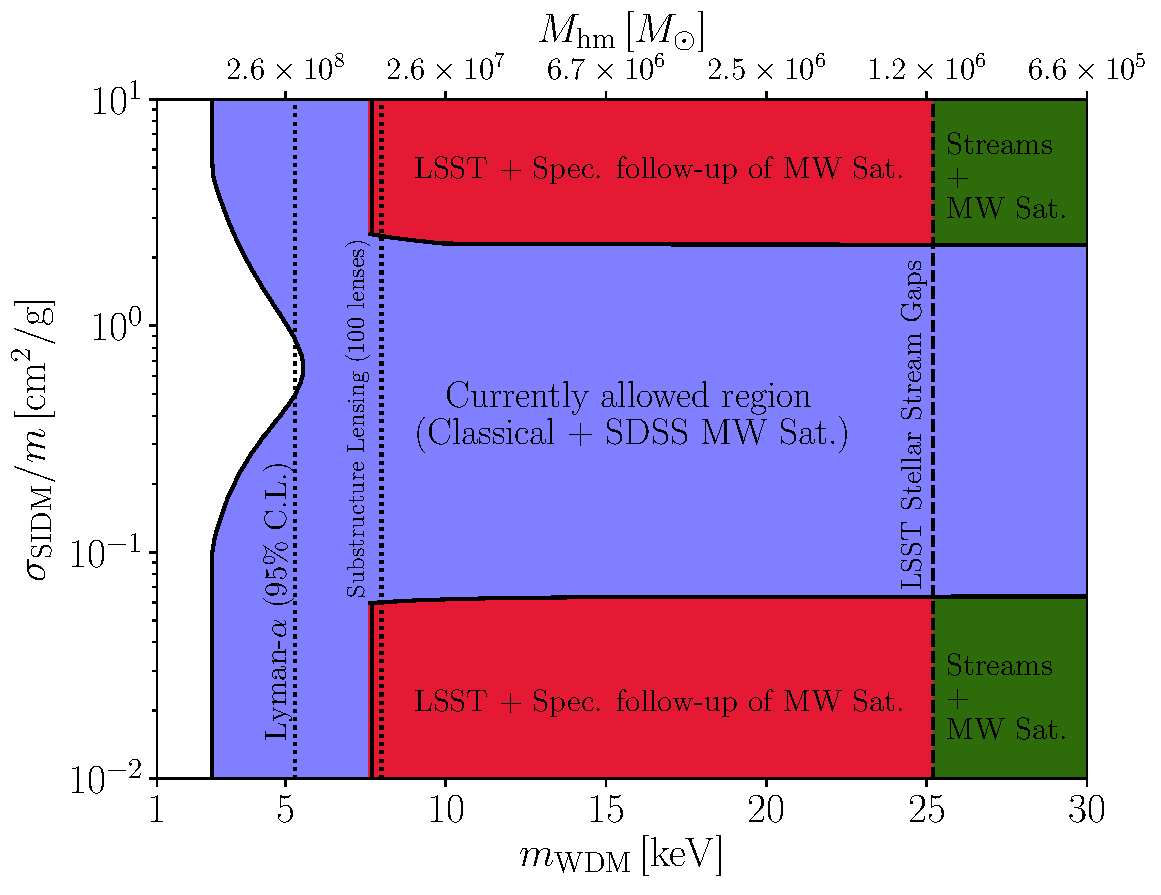
\includegraphics[width=0.75\columnwidth]{figures/SIDM_WDM_figw_coll.pdf}
\caption{\label{fig:sidm_wdm} Projected joint sensitivity to WDM particle mass and SIDM cross section from LSST observations of dark matter substructure. 
The red region is ruled out at 95\% confidence level by current observations of the Milky Way satellite population (the dashed part of the contour is subject to uncertainties due to core collapse, see main text).
The dashed vertical lines correspond to current constraints on the minimum WDM mass from the \Lya forest \citep{2017PhRvD..96b3522I}, and the projected sensitivity of LSST-discovered strong lenses and stellar streams.
%LSST will be sensitive to deviations from the standard CDM scenario through several different probes.
The discovery of additional Milky Way satellites with LSST and their subsequent spectroscopic follow-up will probe the region in blue.
The region with large SIDM cross section delimited by the dashed line labelled ``MW Sats core collapse'' is likely to be probed by Milky Way satellite galaxies, but the simple analysis performed here is insufficient to quantify its sensitivity due to halo core collapse in this regime \citep{Nishikawa:2019lsc}. 
We caution that the exact shape of this region will depend on the amount of tidal disruption that subhalos experience.  
The top axis displays the corresponding half-mode mass as per Eq.~\eqref{eqn:Mhm}. 
Note that $\sigmaSIDM$ stands for the self-interaction cross section evaluated at velocities relevant for Milky Way satellite galaxies ($v_{\rm rel}\sim5$--$50 \kms$). }
\end{figure}

Using the mapping from $L_\star$ and halo mass to $M_{\rm vir}$, our summary statistic can be computed using the expression:
\begin{align}\label{eq:Nsat_above_thresh}
 N_{\rm sat}(L_\star>L_{\rm lim}, \sigma_\star> \sigma_{\star,\rm lim}) &=  \int_{L_{\rm lim}} dL_\star \int_{\sigma_{\star,\rm lim}} d\sigma_\star \int dM_{\rm vir} \frac{dn}{d M_{\rm vir}} P(L_\star|M_{\rm vir}) \\ \nonumber
 &\qquad\qquad \qquad \times \delta\left(\sigma_\star-\bar{\sigma}_\star(\rho_0,c(M_{\rm vir};\mWDM))\right),
\end{align}
where $dn/dM_{\rm vir}$ is the redshift zero subahlo mass function (which depends on $\mWDM$) and $\delta$ is the Dirac delta function. Given values of $\mWDM$ and $\sigmam$, we can use Eq.~\eqref{eq:Nsat_above_thresh} to compute the number of Milky Way satellites observable with LSST that have stellar dispersion above our chosen threshold. As in \secref{smallest_galaxies},
we take $M_V=0$ mag and $\mu=32$ mag/arcsec$^2$ as our detection threshold for LSST, and set $\sigma_{\star,\rm lim}=2.6 \kms$. This latter choice is driven by the minimum stellar dispersion value obtained in our mock observation of satellite galaxies passing the LSST detection threshold as described above, assuming standard CDM. Since measuring stellar dispersions will require spectroscopic follow-up of LSST-discovered satellite galaxies, we fold in our analysis the probability that a given target can be followed up with 30-meter class telescopes given its luminosity and heliocentric distance, as provided in \secref{spectroscopy}.

The resulting projected joint sensitivity to the WDM particle mass and the SIDM cross section are shown in \figref{sidm_wdm}. 
The red region to the left of the figure is already excluded by observations of known classical and SDSS-discovered Milky Way satellites. 
The dashed vertical lines show current constraints from the \Lya forest \citep{2017PhRvD..96b3522I} and the projected sensitivity of strongly lensed systems and stellar streams discovered by LSST.
In blue, we show the region of SIDM-WDM parameter space that would be probed by LSST+spectroscopic measurements of the Milky Way satellite population. 
In the white region at low SIDM cross sections, the central core caused by self-interaction is too small to significantly affect the dynamics of the satellites. In the blue region at high cross sections delimited by the dashed line, tidally-stripped subhalos may undergo core collapse and may thus have similar stellar dispersion to their CDM counterparts, resulting in a loss of sensitivity to the SIDM cross section from the simple statistics given in Eq.~\eqref{eq:Nsat_above_thresh}. However, we note that the expected diversity of the Milky Way satellite population within this region of dark matter parameter space \citep{Nishikawa:2019lsc} is likely to be distinguishable from that predicted by CDM, and we thus include it in the parameter space that LSST can probe. While not shown in \figref{sidm_wdm}, complete gravothermal collapse and subhalo evaporation at very high SIDM cross section ($\gtrsim 10\cmg$) likely imply that these high values are already ruled out.  We thus see that spectroscopic follow-up of LSST-discovered satellites could significantly improve our knowledge of dark matter physics in the prime parameter space corresponding to $\mWDM \sim 5-15 \keV$ and $\sigmam \sim 0.1-10 \cmg$.
